\item[(a)]
\section*{Task (a)}

\subsection*{Problem Statement}
In the Dual Tone Multiple Frequency (DTMF) method, each of the 16 possible information symbols \( q \in \{0, 1, 2, 3, 4, 5, 6, 7, 8, 9, A, B, C, D, *, \#\} \) is represented by a superposition of two sinusoidal audio signals with different frequencies. The assignment of each symbol to the two frequencies contained in the corresponding audio signal is given in Table 1. The duration of a single symbol is \( 70 \, \text{ms} \), and the audio signals of two symbols are separated by a pause of \( 30 \, \text{ms} \). The file `dtmf.wav` contains a signal consisting of a sequence of DTMF signals corresponding to a sequence of randomly chosen symbols, generated with a sampling frequency of \( f_s = 8 \, \text{kHz} \).

\subsection*{Python Script}
\begin{verbatim}
import numpy as np
import matplotlib.pyplot as plt
from scipy.io import wavfile
import os

# Create fig directory if it doesn't exist
if not os.path.exists('fig'):
    os.makedirs('fig')

# Read the DTMF signal from the WAV file
fs, signal = wavfile.read('dtmf.wav')

# Define the duration of the segment to plot (300 ms)
segment_duration = 0.3  # seconds
segment_samples = int(segment_duration * fs)

# Extract the segment
segment = signal[:segment_samples]

# Plot the segment
time = np.arange(segment_samples) / fs
plt.figure(figsize=(10, 6))
plt.plot(time, segment)
plt.title('300 ms Segment of DTMF Signal')
plt.xlabel('Time (s)')
plt.ylabel('Amplitude')
plt.grid(True)
plt.savefig('fig/ex4_a_dtmf_segment.png')
plt.show()

# Perform a Fourier Transform to identify the frequencies
frequencies = np.fft.fftfreq(segment_samples, 1/fs)
spectrum = np.fft.fft(segment)

# Plot the magnitude spectrum
plt.figure(figsize=(10, 6))
plt.plot(frequencies[:segment_samples // 2], np.abs(spectrum[:segment_samples // 2]))
plt.title('Magnitude Spectrum of the DTMF Signal Segment')
plt.xlabel('Frequency (Hz)')
plt.ylabel('Magnitude')
plt.grid(True)
plt.savefig('fig/ex4_a_dtmf_spectrum.png')
plt.show()
\end{verbatim}

\subsection*{Plot of 300 ms Segment}
\begin{figure}[h]
    \centering
    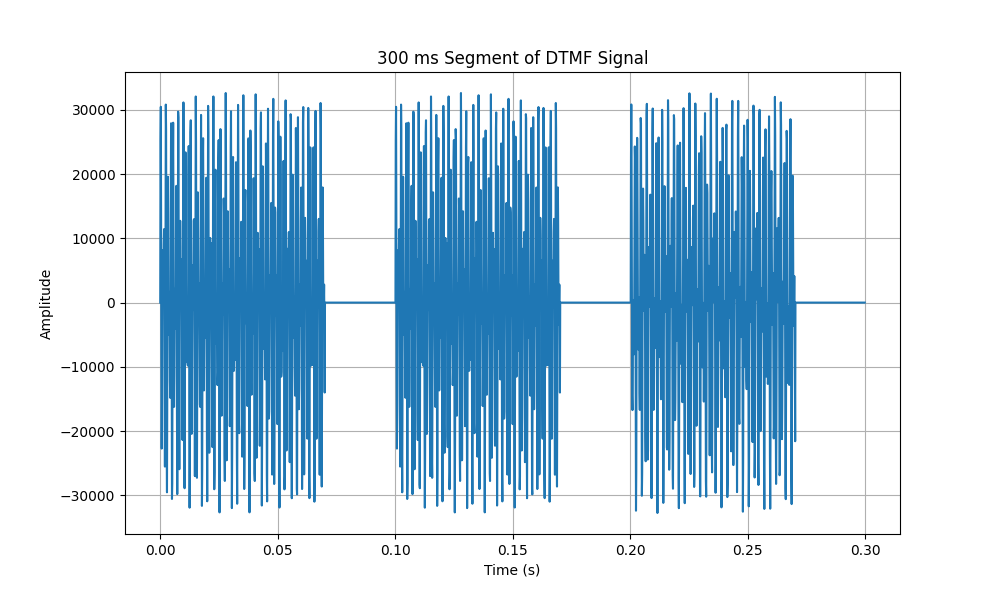
\includegraphics[width=0.8\textwidth]{fig/ex4_a_dtmf_segment.png}
    \caption{300 ms Segment of DTMF Signal}
    \label{fig:ex4_a_dtmf_segment}
\end{figure}

\subsection*{Magnitude Spectrum of the DTMF Signal Segment}
\begin{figure}[h]
    \centering
    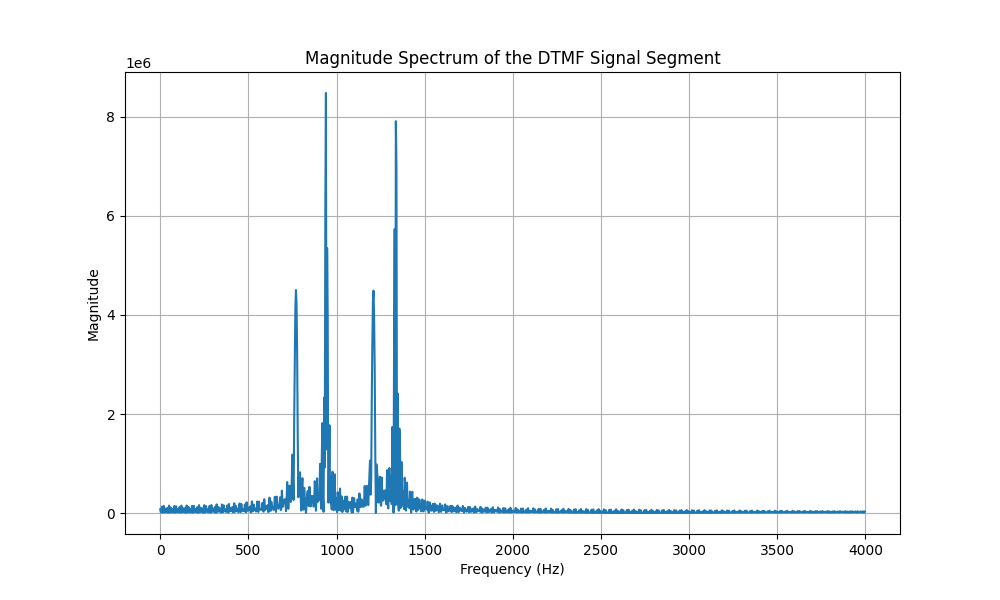
\includegraphics[width=0.8\textwidth]{fig/ex4_a_dtmf_spectrum.png}
    \caption{Magnitude Spectrum of the DTMF Signal Segment}
    \label{fig:ex4_a_dtmf_spectrum}
\end{figure}

\subsection*{Analysis}
Given the segment of the signal in the time domain and its corresponding magnitude spectrum, we can identify the frequencies present in the segment. The frequencies in the DTMF signals correspond to specific symbols as listed in Table 1. By identifying the prominent frequencies in the spectrum, we can determine which symbols are contained in this segment.
